\section{The history of commuting}\label{sec:the-history-of-commuting}

The problem of choosing public commuting, private commuting or moving closer to one's place of work is a more modern
problem.
People have been commuting since the beginning of humanity - from fetching berries in the forest to traveling to
fight in wars.
In more recent human history commuting encapsulates something more complex.
Before the information age in the 20th century and before cars and buses and such were mainstream transport vehicles,
most people traveled on foot or were accompanied by some animal suited for travel to and from work.
This trend reversed as cars and other more technologically advanced vehicles became accessible.
In the early 19 hundred Netherlands, as described in the book ``No bicycle, No bus, No job'', people would flock to the
cities to avoid unemployment as the industrial evolution was in full force.
As most workers were from a lower socioeconomic class with limited resources to spend on transport and luxury, it only
made sense for workers to move closer to the factory they worked at to save time and money~\cite{bek2022}.

\subsection{Technological breakthroughs}\label{subsec:technological-breakthroughs}

As the Netherlands, as well as most other European countries, experienced the same technological breakthroughs in the
same relative timeframes in history, the country is in broad sense comparable to Denmark.
As cars and buses and such populated the streets in the 19 hundreds, commuting slowly became the complex issue we
know it as today.
The escalation of the big cities throughout the 20th century also brought higher education for the people.
The number of people completing higher education in the last 50 years is considerably higher than it was in the
beginning of the 20th century as seen in Figure \ref{fig:education-dk}.

\begin{figure}
    \centering
    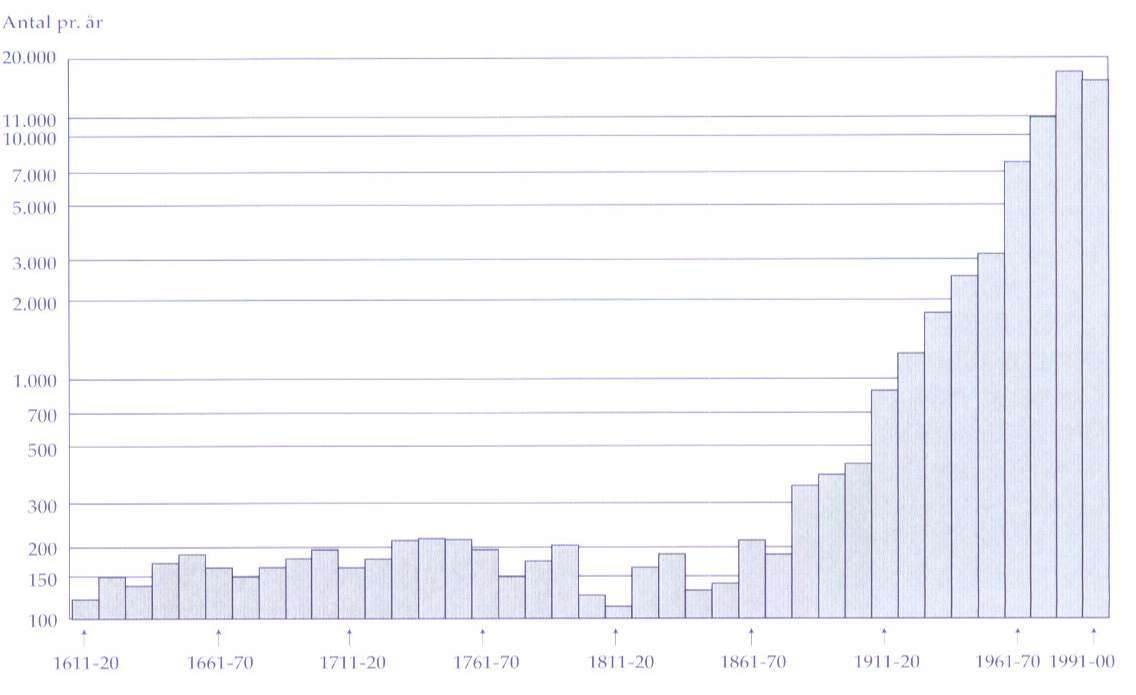
\includegraphics[width=\textwidth]{education-levels}
    \caption{Historical education levels in Denmark~\cite{johansen2005}.}
    \label{fig:education-dk}
\end{figure}

This trend of higher education played a part in the acceleration of technological advancement in society, improving
quality of life of the working class.
With this improvement, more money became available to the working and upper class.
Even though quality of life has improved consistently, the Gini coefficient in Denmark has risen 7.7 percentage points
since 1987~\cite{cepos2023}.
This development has played a significant role in the lack of affordable housing and living in the big cities forcing
working class people to move out of the cities they work in to be able to afford stable housing.
As the big cities still need unskilled and skilled workers in its facilities, the problem of the commuting arises.

Commuting in the rural areas of the country is heavily influenced by cars, as the population density is dramatically
lower there compared to in the big cities~\cite{mulacic2020}.
As a comparison, the present Copenhagen region encapsulates 35\% of the
population while only occupying 7\% of the land area in Denmark~\cite{nielsen&lemberg2017}.
This results in heavy reliance on public transport in big cities, as roads are not big enough for everyone to drive a
car to work every day as opposed to less populated areas where the roads have the capacity for everyone to commute via
car.

\subsection{Public transport in Copenhagen region}
\label{subsec:the-history-of-public-transport-in-copenhagen-region}

Public transport is therefore a part of the equation when it comes to the commuters' preferences.
This has not always been the case, as public transport in the 19 hundreds was lackluster, unreliable and scarce.
The working norm, after the industrial revolution had officially settled into society, was very much controlled by the
factory owners, who demanded specific working hours for their employees.
This resulted in congestion when arriving at work and similar congestion when going home again~\cite{bek2022}.

In today's day, many sectors and businesses have different working hours.
Some are set in stone for obvious reasons, such as hospitals.
Others such as office workers and other officers are just required to work 7 to 8 hours of work per day, regardless of
when this work is performed.
Some jobs are even possible to do from home due to the internet and technological advancements.
This evolution of this work environment in history has made it possible for a worker to work in the city, while living
in the suburbs through commuting or working from home.
All these scenarios, whether you are living in the city or in the suburbs, and whether you are working in the city or
in the suburbs it needs to be encapsulated into our program to properly include every scenario and thereby expanding the
use cases of our program.
